\documentclass[]{interact}

%\usepackage[caption=false]{subfig}% Support for small, `sub' figures and tables
%\usepackage[nolists,tablesfirst]{endfloat}% To `separate' figures and tables from text if required
%\usepackage[doublespacing]{setspace}% To produce a `double spaced' document if required
%\setlength\parindent{24pt}% To increase paragraph indentation when line spacing is doubled
%\setlength\bibindent{2em}% To increase hanging indent in bibliography when line spacing is doubled

\usepackage[numbers,sort&compress]{natbib}% Citation support using natbib.sty
\bibpunct[, ]{[}{]}{,}{n}{,}{,}% Citation support using natbib.sty
\renewcommand\bibfont{\fontsize{10}{12}\selectfont}% Bibliography support using natbib.sty

\usepackage{amsmath}
\usepackage{algorithm}
\usepackage{algpseudocode}
\usepackage[T1]{fontenc}
\usepackage{pgfplots}
\usetikzlibrary{arrows}
\pgfplotsset{compat=1.16}
\usepackage{caption}
\usepackage{subcaption}
%\usepackage{minted}

\usepackage[hidelinks]{hyperref}

\theoremstyle{plain}% Theorem-like structures provided by amsthm.sty
\newtheorem{theorem}{Theorem}[section]
\newtheorem{lemma}[theorem]{Lemma}

\newtheorem{corollary}[theorem]{Corollary}
\newtheorem{proposition}[theorem]{Proposition}

\theoremstyle{definition}
\newtheorem{definition}[theorem]{Definition}
\newtheorem{example}[theorem]{Example}

\theoremstyle{remark}
\newtheorem{remark}{Remark}
\newtheorem{notation}{Notation}

\newcommand{\RR}{\mathbb{R}}

\newcommand{\eps}{\epsilon}
\newcommand{\grad}{\nabla}
\newcommand{\Div}{\nabla\cdot}

\newcommand{\cK}{\mathcal{K}}
\newcommand{\cX}{\mathcal{X}}

\begin{document}

%\articletype{ARTICLE TEMPLATE}% Specify the article type or omit as appropriate

\title{Adaptive mesh refinement for locating free boundaries in obstacle problems}

\author{
\name{G.~Stefano Fochesatto\thanks{CONTACT G.~Stefano Fochesatto Email: gsfochesatto@alaska.edu} and Ed Bueler}
\affil{Dept.~of Mathematics and Statistics, University of Alaska Fairbanks, USA}
}

\maketitle

\begin{abstract}
Free-boundary problems posed as variational inequalities, such as obstacle problems, appear in many scientific and engineering applications.  In the finite element (FE) solution of these problems, the geometrical error in locating the unknown free boundary, equivalently in locating the active and inactive sets, often dominates the overall numerical error.  In this paper we propose, and implement using the Firedrake FE library, adaptive mesh refinement (AMR) strategies which enhance the mesh resolution around the free boundary.  These methods mark elements for refinement based on a computed solution; refinement then reduces numerical errors while controlling the growth of mesh complexity.  We consider three AMR methods of this type: (i) an unstructured dilation operator based on discrete adjacency to the computed free-boundary; (ii) a variable-coefficient diffusion method which thresholds a diffused active set indicator function; and (iii) a metric-based method which averages an anisotropic, Hessian-derived Riemannian metric with an isotropic metric computed from the diffused active set indicator.  The methods are evaluated by norm error and geometrical error in active set localization, the latter using Jaccard and Hausdorff distances.  Certain hybrid strategies are then considered.  Applications include the classical Poisson obstacle problem and a shallow ice flow problem for predicting the glaciated region in a mountain range.
\end{abstract}

%\begin{keywords}
%FIXME
%\end{keywords}


\section{Introduction} \label{sec:intro}

The classical obstacle problem \cite{KinderlehrerStampacchia1980} finds the equilibrium position (vertical displacement) $u$ of an elastic membrane, attached to a fixed boundary, with some applied force $f$, but where the membrane is constrained to lie above some obstacle $\psi$.  Let $\Omega \subset \RR^d$ be a bounded, open domain, with the data $f$ and $\psi$ given on $\Omega$.  The strong formulation of this problem is a complementarity problem (CP).  It gives conditions satisfied by the solution $u$ almost everywhere in $\Omega$:
\begin{subequations} \label{eq:classical:ncp}
\begin{align}
  -\nabla^2 u - f \geq 0 \label{eq:classical:ncp:a} \\
  u - \psi \geq 0\\
  (-\nabla^2u - f)(u - \psi) = 0 \label{eq:classical:ncp:c}
\end{align}
\end{subequations}
From a solution to \eqref{eq:classical:ncp} we may identify the inactive and active sets,
\begin{equation}
  I_u = \{x \in \Omega \,:\, u(x) > \psi(x)\}, \quad A_u = \Omega \setminus I_u. \label{eq:classical:sets}
\end{equation}
The free boundary $\Gamma_u = \Omega \cap \partial I_u$ is where $I_u$ meets $A_u$ within $\Omega$.  From \eqref{eq:classical:ncp}, $u$ solves the Poisson equation $-\nabla^2u = f$ on $I_u$, while both Dirichlet ($u=\psi$) and Neumann ($\grad u = \grad \psi$) conditions apply along $\Gamma_u$.  An example is shown in Figure \ref{fig:ball}, in which $A_u$ is the closed disc of contact ($u=\psi$), and $\Gamma_u$ is a circle.

\begin{figure}[H]
\centering
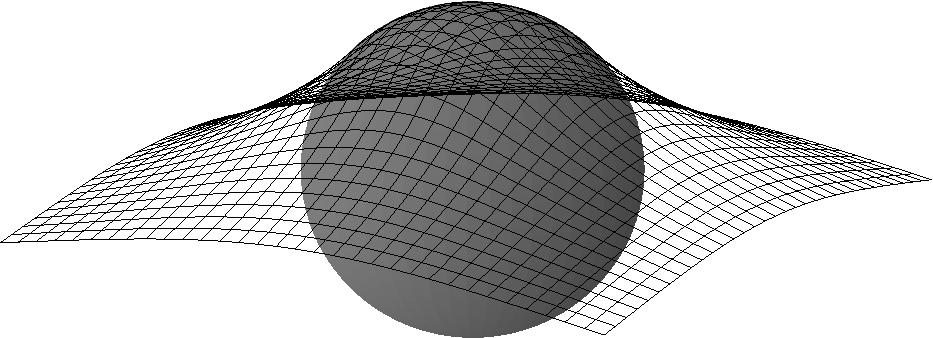
\includegraphics[width=0.7\textwidth]{static/obstacle65.pdf}
\caption{Solution $u$ of a classical obstacle problem; the obstacle $\psi$ is the upper hemisphere of a ball.}
\label{fig:ball}
\end{figure}

As is well-known, CP \eqref{eq:classical:ncp} has a weak formulation which is a variational inequality (VI) over a Sobolev space.  Let $\cX=H^1(\Omega)$ \cite{ElmanSilvesterWathen2014} and suppose $\psi \in X \cap C(\bar\Omega)$.  Let $g:\partial \Omega\to \RR$ be continuous, also satisfying $g \ge \psi|_{\partial \Omega}$.  Let
\begin{equation} \label{eq:classical:admissible}
\cK = \{u \in \cX \,:\, u \ge \psi \text{ and } u|_{\partial \Omega} = g\}
\end{equation}
be the admissible set for solutions, a closed and convex subset of $X$.  For $f\in L^2(\Omega)$, the VI formulation of the obstacle problem \cite{KinderlehrerStampacchia1980} is then to find $u\in \cK$ so that
\begin{equation} \label{eq:classical:vi}
\int_\Omega \nabla u \cdot \nabla(v - u) \ge \int_\Omega f(v - u) \quad \text{ for all } v \in \cK.
\end{equation}

Section \ref{sec:vifem} will recall some of the theory of such VIs, and their finite element (FE) approximation.  The conforming FE approximation of \eqref{eq:classical:vi} uses the same weak form but over the discrete space.  As for PDEs \cite{ElmanSilvesterWathen2014}, because the exact solution $u$ and the FE solution $u_h$ solve VIs, with the latter computed on a mesh with characteristic size $h>0$, the norm errors $\|u-u_h\|$ can be bounded, and related to the approximation properties of the FE space.  Specifically, an extension of the Falk \cite{Falk1974} technique for \emph{a priori} norm error estimation for VIs is provided in Section \ref{sec:vifem}.

However, the geometrical mesh error in locating the free-boundary $\Gamma_u$, by itself, largely explains the behaviour of the numerical error.  (This fact is only weakly acknowledged in the FE literature for VIs \cite[for example]{Suttmeier2008}.)  For example, to make this clear in one dimension suppose $\Omega = (-1,1)$, $\psi(x)=0.5 - x^2$, and $g=0$.  The exact solution $u$ of \eqref{eq:classical:vi} is easily calculated, with free boundaries at $x_*=\pm(2-\sqrt{2})/2$ (Figure \ref{fig:parabola}).  Suppose our FE approximation uses piecewise-linear elements and uniform meshes, and let $\Delta_h$ be the minimum distance between a nodal coordinate and $x_*$, over a uniform mesh.  Because the values $x_*$ are irrational, the mesh nodes will never coincide exactly with $x_*$, and $\Delta_h$ will be an erratic function of $h$, though $\Delta_h = O(h)$.  Figure \ref{fig:parabola} (right) compares the $H^1$ and $L^2$ norm errors $\|u-u_h\|$ to $\Delta_h$.  We see that the purely-geometrical error $\Delta_h$, in approximating the free boundary, fully explains the erratic behavior of the norm errors.

\begin{figure}[H]
\mbox{
\begin{minipage}[t]{0.45\textwidth}
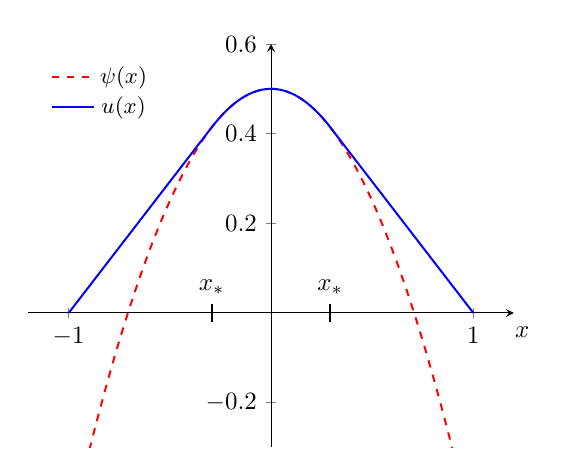
\begin{tikzpicture}[scale=0.9]
    \begin{axis}[
      axis lines = middle,
      xlabel = {$x$},
      xlabel style = {at={(1.05, 0.25)}},  % relative to whole figure box [0,1]x[0,1]
      domain = -1:1,
      samples = 100,
      xmin = -1.2,
      xmax = 1.2,
      ymin = -0.3,
      ymax = 0.6,
      xtick = {-1,1},
      legend pos = north west,
      legend style = {draw=none, font=\small}
    ]
      % Parameters
      \def\b{(2-sqrt(2))/2}
      \def\a{-\b}
      % Plot the obstacle function psi(x)
      \addplot[
        thick,
        red,
        dashed
      ] {0.5 - x^2};
      \addlegendentry{$\psi(x)$}
  
      % Plot u(x) in three pieces
      \addplot[
        thick,
        blue,
        domain=-1:\a
      ] {((.5 - \a*\a)/(\a + 1))*(x + 1)};
      \addplot[
        thick,
        blue,
        domain=\a:\b
      ] {0.5 - x^2};
      \addplot[
        thick,
        blue,
        domain=\b:1
      ] {-((.5 - \b*\b)/(1 - \b))*(x - 1)};
      \addlegendentry{$u(x)$}

      % indicate free boundary locations
      \addplot[black, thick, draw] coordinates {(\a,-0.02) (\a,0.02)} node[above] (A) {$x_*$};
      \addplot[black, thick, draw] coordinates {(\b,-0.02) (\b,0.02)} node[above] (B) {$x_*$};
    \end{axis}
  \end{tikzpicture}
  
\end{minipage}
\quad
\begin{minipage}[t]{0.55\textwidth}
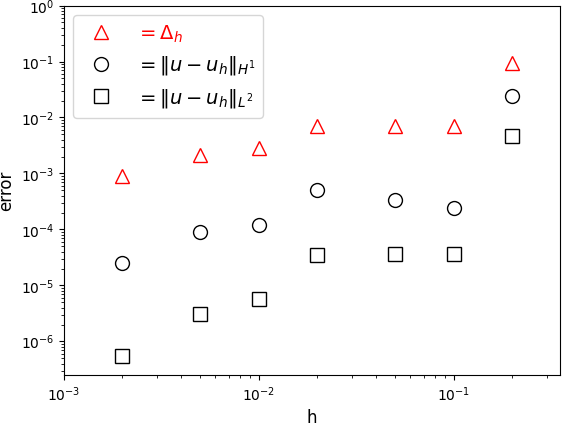
\includegraphics[width=0.9\textwidth]{static/VIConvergence.png}
% FIXME regenerate with labels ||u-u_h||_{H^1} = O(h^1.09), ||u-u_h||_{L^2} = O(h^1.57), \Delta_h
\end{minipage}
}
\caption{Left:  A one-dimensional obstacle problem with a parabolic obstacle and known free boundary locations $x_*$.  Right:  The geometrical free-boundary error $\Delta_h$ explains the erratic error norm $\|u-u_h\|$ behavior.}
\label{fig:parabola}
\end{figure}

Our numerical results (Section \ref{sec:results}), along with the above example, justify our somewhat-heuristic approach to adaptive mesh refinement (AMR) for VIs.  Because the convergence of VI problems is dominated by the error in approximating the free boundary, an adaptive refinement scheme that is quickly able to concentrate effort around the solution free boundary will both enhance convergence to the solution over the inactive set, and reduce unnecessary computation in the active set.  This approach is especially valuable in applications where a large portion of the domain is active set, and thus where no numerical approximation of the operator is actually required; the glacier example in Section \ref{sec:app} is such an application.

Note that while the classical obstacle problem in form \eqref{eq:classical:vi} is equivalent to constrained minimization of a scalar objective defined on $X$ \cite{KinderlehrerStampacchia1980}.  However, the analysis of FE errors for VI problems does not require such an objective, and for example in Section \ref{sec:app} no such objective exists.  Thus we will not directly consider any optimization principle.

Also note that the current paper considers only meshs of triangles or tetrahedra, and $P_1$ elements (Section \ref{sec:results}), and so only $h$-refinement is addressed.  VIs can be solved using higher-order elements if nontrivial monotonicity modifications are made \cite{KeithSurowiec2024}, but this is not attempted here.

Three AMR methods are described in Section \ref{sec:viamr}.  Our implementations of these methods use the Firedrake finite element library and produce conforming meshes with no hanging nodes.  Two methods are of the tag-and-refine type, only differing by the analysis technique used to identify which elements to tag.  For these methods skeleton-based refinement \cite{PlazaCarey2000} is applied after tagging, as implemented within PETSc's DMPlex component \cite{petsc-user-ref}.

The third method is goal-oriented and metric-based \cite{Alauzet2010,Wallworketal2020}.  This method constructs an intermediate representation of the size, shape, and orientation of the refinement, namely a tensor-valued Riemannian metric, and then the mesh is actually refined using the MMG mesh library \cite{DapognyDobrzynskiFrey2014}.

% PROBABLY NOT NEEDED: Traditional AMR for PDE problems \citep{BangerthRannacher2003} computes error indicators within the solution domain based on analysis of an FE solution computed on the current mesh.  These methods are designed to increase mesh resolution or polynomial degree \cite{Demkowicz2007} by means of a local error estimator, for some goal, the quantity of interest $J(\cdot)$. The dual weighted residual (DWR) method \cite{RannacherSuttmeier1997} begins with a posteriori or a priori analysis of the quantity $J(u) - J(u_h)$.  Estimates of this error quantity are then decomposed into local element-wise error estimators which can be used as a heuristic to tag elements for refinement.

The constraint of $u \geq \psi$ makes VI problems nonlinear (even if the operator is linear).  Thus an iterative solver is required.  Our solver is a VI-adapted Newton method with a reduced-space line search (RSLS) \cite{BensonMunson2006}, implemented in PETSc \cite{petsc-user-ref}.  Such a numerical method does not converge until the active and inactive sets stabilize on the given mesh, so that the discrete free boundary is identified.  Upon stabilizaiton, the domain of quadratic convergence can be entered, giving convergence in a few more iterations.  Newton solvers like RSLS can therefore only adjust the approximated free boundary by one-cell per iteration \citep{GraeserKornhuber2009}, and overall convergence is roughly proportional to the number of grid spaces between the initial iterate free boundary and the solution free boundary \citep{Bueler2021}.  Using the meshes generated here as coarse grids for a multilevel solver, for example the FASCD solver in \cite{BuelerFarrell2024}, is one path to a scalable solution process for VIs.

In the first method from Section \ref{sec:viamr}, which we call the variable-coefficient diffusion (VCD) method, we compute a node-wise indicator function for the active set for use as an initial iterate in a single step of a time-dependent heat equation problem.  Solving a single step of this problem has the effect of smoothing the indicator about the free boundary.  The smoothed result is then averaged over each element and thresholded for refinement tagging.

The second method, called unstructured diffusion operator (UDO), focuses on the discrete identification of elements adjacent to the free boundary, employing a graph-based approach to mark neighboring elements for refinement.  This generalizes the bitmap image processing operation of dilation [cite] to unstructured meshes.

FIXME 3RD METHOD

FIXME The remaining material is organized as follows.  We give a brief background on solving VIs numerically.  Via a 1D example, we illustrate why the error arising from the geometric error in approximating the free boundary dominates the overall numerical error.   Then we introduce the two new adaptive refinement schemes for VIs, VCES and UDO, and provide a detailed description of their implementations.  The results section demonstrates the effectiveness of the proposed methods in enhancing mesh resolution around free boundaries. 

FIXME TABLE OF ACRONYMS


\section{Variational inequalities and their finite element approximation} \label{sec:vifem}

In this section we summarize some basic theory of the VI formulation of unilateral obstacle problems in Banach spaces.  Under a hypothesis of coercivity we have continuum well-posedness even for nonlinear operators.  Our extension of the Falk \cite{Falk1974} technique for VIs, which generalizes Cea's lemma \cite{ElmanSilvesterWathen2014} for PDE problems, then gives an upper bound on the FE norm error, and a convergence argument.  The same Falk-type inequality illuminates why targeted mesh refinement around the free boundary provides improved solutions.

For a bounded, open domain $\Omega \subset \RR^d$, $d=2,3$, with Lipschitz boundary \cite{Ciarlet2002}, let $\cX = W^{1,p}(\Omega)$, $p>1$, be the Sobolev space of measurable functions with $p$th-integrable gradients \cite{Evans2010}, with norm denoted $\|\cdot\|$.  For simplicity we will assume continuous problem data, possessing well-defined point values, so suppose $\psi \in \cX \cap C(\bar\Omega)$, and assume $g\in C(\partial \Omega)$ satisfies $g \ge \psi|_{\partial\Omega}$.  As for the classical obstacle problem \eqref{eq:classical:admissible}, let
\begin{equation} \label{eq:admissible}
\cK = \{v \in \cX \,:\, v \ge \psi \text{ and } v|_{\partial \Omega} = g\}
\end{equation}
be the admissible subset.  Note that $\cK\subset \cX$ is closed and convex, and also that $\psi\in\cK$.

Let $\cX'$ be the dual space of $\cX$, with application of a linear functional denoted $\omega[v] \in \RR$ for $\omega \in \cX'$ and $v\in \cX$, and with norm $\|\omega\|' = \sup_{\|v\|=1} |\omega[v]|$.  Let $F:\cK \to \cX'$ be a given continuous operator (function), generally nonlinear, and let $\ell\in \cX'$ be given.  The VI associated to this data, a unilateral obstacle problem, is to find $u\in \cK$ so that
\begin{equation} \label{eq:vi}
F(u)[v - u] \ge \ell[v - u] \quad \text{ for all } v \in \cK.
\end{equation}
This problem generalizes the classical obstacle problem \eqref{eq:classical:vi}.

The VI problems considered here can be analyzed within the framework of monotonicity and coercivity.  We say $F$ is monotone if $(F(v) - F(w))[v - w] \ge 0$ for all $v,w \in \cK$, and that $F$ is $q$-coercive, for $q>1$, if there is $\alpha>0$ so that
\begin{equation} \label{eq:coercive}
(F(v) - F(w))[v - w] \ge \alpha \|v-w\|^q
\end{equation}
for all $v,w \in \cK$.  Note that if $F$ is $q$-coercive then it is also monotone, indeed strictly monotone in the sense that $(F(v) - F(w))[v - w] > 0$ for $v\ne w$.  It is a well-known fact that if $F$ is continuous and $q$-coercive then VI \eqref{eq:vi} is well-posed \cite[Corollary III.1.8]{KinderlehrerStampacchia1980}.

The classical obstacle problem in weak form, inequality \eqref{eq:classical:vi}, has $\cX=W^{1,2}(\Omega) = H^1(\Omega)$, i.e.~$p=2$, and $F(u)[v] = \int_\Omega \grad u \cdot \grad v$.  Here $F$ is linear and defined on all of $\cX$, while $F$ in \eqref{eq:vi} might be only defined on $K$.  Also $F$ is $2$-coercive in the classical problem, because the (weak) Laplacian is uniformly elliptic \cite{Evans2010}; of course \eqref{eq:classical:vi} is well-posed.  Problem \eqref{eq:classical:vi} is also the first-order optimality condition for the minimization of a continuous, quadratic objective function over the admissible set $\cK$, but as noted earlier we will not need this optimization structure at any point.

Returning to the general case with $\cX = W^{1,p}(\Omega)$ and $p>1$, note that the residual would be zero almost everywhere ($F(u)-\ell=0$) in a PDE case, i.e.~without an inequality constraint.  By contrast, for a VI over $\cK\subset \cX$, defined by \eqref{eq:admissible}, we only know that $F(u)-\ell=0$ a.e.~in the unknown inactive set $I_u$.  On the other hand, although the residual may be highly irregular ($F(u)-\ell\in X'$), in the active set it is at least nonnegative.  Thus the following lemma states a precise complementarity problem associated to the VI weak form \eqref{eq:vi}; compare \eqref{eq:classical:ncp} for the classical obstacle problem.

\begin{lemma} \cite[Theorem 6.22]{KinderlehrerStampacchia1980}. Suppose $u\in \cK$ solves \eqref{eq:vi}.  Then $F(u)-\ell$ is a positive Borel measure $d\mu_u$ supported in the active set $A_u$, and so if $w\in\cX$ then
\begin{equation}
(F(u)-\ell)[w] = \int_{A_u} w\, d\mu_u. \label{eq:measure}
\end{equation}
\end{lemma}

Let $\cX_h \subset \cX \cap C(\bar\Omega)$ be a finite-dimensional FE subspace.\footnote{Not that our FE method is conforming in the PDE sense \cite{ElmanSilvesterWathen2014}, but admissibility for the VI case is more subtle, as seen in stating Theorem \ref{thm:genfalk}.}  For simplicity we will assume that $\partial \Omega$ is polygonal and that there is $g_h\in\cX_h$ such that $g_h=g$ exactly along $\partial \Omega$.  Let $\psi_h \in \cX_h$ be the FE obstacle, assumed to satisfy the compatibility requirement that $\psi_h \le g_h$ along $\partial\Omega$.  Note that $\psi_h$ might be an interpolant or projection of the continuum obstacle $\psi$, but no specific relationship is implied for now.  Define the FE admissible set
\begin{equation} \label{eq:fe:admissible}
\cK_h = \{v_h \in \cX_h \,:\, v_h \ge \psi_h \text{ and } v_h|_{\partial \Omega} = g_h|_{\partial\Omega}\}.
\end{equation}
If also $\psi_h \ge \psi$ then $\cK_h\subset \cK$, but otherwise not; we will consider this issue again below.  Our FE method seeks $u_h\in\cK_h$ such that
\begin{equation} \label{eq:fe:vi}
F(u_h)[v_h - u_h] \ge \ell[v_h - u_h] \quad \text{ for all } v_h \in \cK_h.
\end{equation}

The following theorem generalizes that of Falk \cite{Falk1974}; see also Theorem 5.1.1 in \cite{Ciarlet2002}.  A further generalization, allowing non-conforming operators $F_h\approx F$, is Theorem 6.3 in \cite{Bueler2024}; this adds a fourth term to the bound.

\begin{theorem} \label{thm:genfalk}  For $1<q<\infty$, define the conjugate exponent $q'=q/(q-1)$.  Assume that either $F$ is $q$-coercive over $\cX$, or that $\cK_h\subset \cK$ and $F$ is $q$-coercive over $\cK$, in either case with constant $\alpha>0$.  Assume similarly that either $F$ is Lipschitz on bounded sets of $\cX$ or that $\cK_h\subset \cK$ and $F$ is Lipschitz on bounded subsets of $\cK$.  Suppose $u\in\cK$ solves \eqref{eq:vi} and $u_h\in\cK_h$ solves \eqref{eq:fe:vi}.  Let $R_h=\max\{\|u\|,\|u_h\|\}$.  Then there is a constant $c=c(R_h,\alpha)>0$, not otherwise depending on $u$ or $u_h$, so that
\begin{align}
\|u-u_h\|^q &\le \frac{2}{\alpha} \inf_{v\in\cK} \int_{A_u} (v-u_h)\,d\mu_u \label{eq:falk} \\
   &\quad\, + \frac{2}{\alpha} \inf_{v_h\in\cK_h} \int_{A_u} (v_h-\psi)\,d\mu_u \notag \\
   &\quad\, + c \inf_{v_h\in\cK_h} \|v_h - u\|^{q'}. \notag
\end{align}
\end{theorem}

\begin{proof}  For arbitrary $v\in\cK$ and $v_h\in\cK_h$, rewrite \eqref{eq:vi} and \eqref{eq:fe:vi} as $F(u)[u] \le F(u)[v] + \ell[u-v]$ and $F(u_h)[u_h] \le F(u_h)[v_h] + \ell[u_h-v_h]$.  It follows from these inequalities, and $q$-coercivity of $F$, that
\begin{align}
\alpha \|u-u_h\|^q &\le \left(F(u)-F(u_h)\right)[u-u_h] \label{eq:falkdance} \\
  &= F(u)[u] + F(u_h)[u_h] - F(u)[u_h] - F(u_h)[u] \notag \\
  &\le F(u)[v] + \ell[u-v] + F(u_h)[v_h] + \ell[u_h-v_h] \notag \\
  &\qquad - F(u)[u_h] - F(u_h)[u] \notag \\
  &= F(u)[v-u_h] - \ell[v-u_h] + F(u_h)[v_h-u] - \ell[v_h-u] \notag \\
  &= \left(F(u)-\ell\right)[v-u_h] + \left(F(u)-\ell\right)[v_h-u] \notag \\
  &\qquad + \left(F(u)-F(u_h)\right)[u-v_h] \notag
\end{align}
Since $u,u_h\in B_{R_h} = \{w\in\cX\,:\,\|w\|\le R_h\}$, by the Lipschitz assumption there is $C(R_h)>0$ so that
\begin{equation}
\left(F(u)-F(u_h)\right)[u-v_h] \le C(R_h) \|u-u_h\|\|u-v_h\|. \label{eq:falklip}
\end{equation}
Now use Young's inequality with $\eps>0$ \cite[Appendix B.2]{Evans2010}:
\begin{align}
\alpha \|u-u_h\|^q &\le \left(F(u)-\ell\right)[v-u_h] + \left(F(u)-\ell\right)[v_h-u]  \label{eq:falkyoung} \\
  &\qquad + C(R_h) \left(\eps\|u-u_h\|^q + \tilde C(\eps) \|u-v_h\|^{q'}\right) \notag
\end{align}
where $\tilde C(\eps) = (\eps q)^{-q'/q} {q'}^{-1}$.  Choose $\eps>0$ so that $C(R_h) \eps \le \alpha/2$, and subtract:
\begin{align}
\frac{\alpha}{2} \|u-u_h\|^q &\le \left(F(u)-\ell\right)[v-u_h] + \left(F(u)-\ell\right)[v_h-u]  \label{eq:abstract:five} \\
  &\qquad + C(R_h) \tilde C(\eps) \|u-v_h\|^{q'} \notag
\end{align}
Apply the Lemma, note $u=\psi$ a.e.~in $A_u$, and take infimums to show \eqref{eq:falk}.  Also note that $c=2 C(R_h) \tilde C(\eps)/\alpha$.
\end{proof}

FIXME PDE case

FIXME $\cK_h\subset \cK$ case

FIXME so what: if we have accurate free boundary then \dots and active set apparent errors can be ignored

FIXME compare \cite{Suttmeier2008} re DWR


\section{New adaptive mesh refinement strategies} \label{sec:viamr}

To explain our methods for adaptive mesh refinement for VIs, we will first review certain methods for adaptive mesh refinement from the literature for PDEs.  Tagging methods, are a class of adaptive methods which assess the suitability of a mesh element-by-element in computing a Quantity of Interest (QoI) like $L_2$ error or another post computation functional like drag or lift \cite{bangerth_adaptive_2003}. The main idea behind most tagging methods is the refinement loop:

\begin{algorithm}
  \caption{Tag and refine}
  \begin{algorithmic}
    \State Solve: Solve the PDE on the current mesh. 
    \State Estimate: Estimate the error in the QoI element-by-element.
    \State Tag: Tag elements for refinement based on the error estimate.
    \State Refine: Refine or coarsen the mesh maintaining the minimum angle criteria.
  \end{algorithmic}
\end{algorithm}

Throughout the literature (\citet{becker_feed-back_1996}, \citet{bangerth_adaptive_2003}, \citet{suttmeier_numerical_2008}) one finds a variety of ways to perform the "Estimate" step. As we mentioned in the Introduction a common way is by the Dual Weighted Residual (DWR) method introduced in \citet{becker_feed-back_1996}. For further details see \citet[Chapter 3]{bangerth_adaptive_2003}. A general approach for extending the DWR method to variational inequalities can be found in \citet{suttmeier_numerical_2008}.  However, the methods proposed here are not based on the DWR method. 

There are also several ways to perform the "Tag" step. Consider the following fixed-rate strategy found in \citet[Chapter 4]{bangerth_adaptive_2003}. For fractions $X, Y$ with $1 - X > Y$ and a mesh with $N$ elements, refine the $X\cdot N$ elements with the largest error indicator and coarsen the $Y\cdot N$ elements with the smallest error indicator. For appropriate choices of $X$ and $Y$ this has the effect of keeping the degrees of freedom almost constant. There are other more exotic solutions which accomplish different goals. For example there is a fairly impractical "error-balancing" strategy also described in \citet[Chapter 4]{bangerth_adaptive_2003} which seeks to equilibrate the error indicators across the mesh.

The "Refine" step in Algorithm 2 addresses to refine cells once they have been selected for refinement. This process involves two considerations: maintaining the minimum angle condition and managing hanging nodes. As illustrated in Figure 2.4, elements can be refined in such a way that the minimum angle condition is violated, leading to poor convergence properties. The second issue concerns hanging nodes, which are nodes that do not have a "covering" relation to all neighboring elements; this concept will be elaborated on further.

A tagging strategy like the one above can be implemented in Firedrake using Netgen/NGSolve integration \citep{zerbinati_ngspetsc_nodate}.  This integration brings several new features to Firedrake, but for our purposes the most important is the \texttt{refine\_marked\_elements()} method.  This method resides inside of a netgen mesh object and takes an indicator function over the domain representing which elements are marked for refinement. This method is capable of dealing with hanging nodes by use of transition cells

The operation of interpolating a function into a DG0 space is central to our proposed methods for adaptive refinement. Conceptually this operation allows us to compute estimators (Estimate step of Algorithim 2) which take on a single value over vertices and then convert them, by averaging over an element into an estimator which takes on a single value over the element. Averaging a function over elements is equivalent to interpolation into a DG0 space. To see this, consider the definition of the interpolation operation given in the Firedrake user manual \citep{ham_firedrake_2023}. 
Let $u$ be a function over some domain $\Omega$ and $V$ be a finite element space defined on $\Omega$ with basis $\{\phi_i\}_{i = 1}^N$. Then $interpolate(u, V)$ is given by $\sum_{i = 1}^N v_i \phi_i$ where $v_i = \phi^*_i$ and $\phi^*_i$ is an element of the dual basis of $V$. (Recall that the dual basis of $V_\Omega$ is given by the vector $\{\phi^*_i\}$, such that $\phi^*_i(\phi_j) = \delta_{ij}$). The corresponding dual basis vector of a DG0 space is the following average
\begin{equation}
  \phi_j^*(f) = \frac{1}{area(\triangle_j)}\int_{\triangle_j} f\, dx.
\end{equation}
Note that this choice of functional has the property that $\phi^*_i(\phi_j) = \delta_{ij}$. Now $interpolate(u, V) = \sum_{i = 1}^n v_i\theta_i$ where
\begin{equation}
  v_i = \frac{1}{area(\triangle_i)}\int_{\triangle_i} u \, dx.
\end{equation}

We propose two strategies for adaptive refinement of variational inequalities, which we call Variable Coefficient Elliptic Smoothing (VCES) and Unstructured Dilation Operator (UDO). These methods are designed to enhance mesh resolution at the free boundary found when solving the VI. These methods are the Estimate and Tag steps in Algorithm 2. They effectively control the error associated with approximating the free boundary, as observed in Section 3.3 and illustrated in Figure 3.4. Note that Firedrake/Netgen is used for the Solve and Refine steps in Algorithim 2.

The first strategy is called Variable Coefficient Elliptic Smoothing (VCES). The idea is to use the residual $u^k - \psi$ and a positive tolerance to construct $s_0$, a node-wise indicator function for the active set. This indicator function is used as the initial condition of a variable-coefficient and time-dependent heat equation problem which has the effect of smoothing this indicator near the free boundary. This heat equation problem is solved for a single timestep via implicit Euler, the result of which, we'll call $s_1$. This problem is a linear elliptic PDE, hence "elliptic smoothing"
\begin{equation}
  \frac{1}{\Delta t}(s_1 - s_0) = \nabla^2 s_1.
\end{equation}
Our choice of timestep $\Delta t_i = \frac{1}{2}(\text{avg}(\text{diam}(\triangle_i)))^2$ where $\triangle_i$ is the set of all elements incident to vertex $i$. This choice depends on the element, thus "variable coefficient". Varying the timestep based off of neighboring element diameter has the effect of applying the same amount diffusion across all elements regardless of size. The result is then interpolated into a DG0 space and thresholded to produce the refinement indicator, as in Algorithim 2. There are various parameters to consider with this technique. The choice of timestep and thresholding parameters will substantially affect the "distance" about which the free boundary is resolved. 

\begin{algorithm}[H]
	\caption{Variable Coefficient Elliptic Smoothing Element Tagging for VIs}\label{alg:cap}
	\begin{algorithmic}[1]
		\Require $tol \in \mathbb{R}$, $u^k \in K_\psi, \psi \in V$, $W$ is DG0 FE space.
		\Require Threshold parameters $0\leq \alpha < \beta \leq 1$.
		\State Compute the nodal active set indicator function $s_0$
		  \begin{equation*}
			s_0 = \begin{cases}
			  1 & \text{ if } u^k - \psi < tol\\
			  0 & \text{ otherwise}
			\end{cases}
		  \end{equation*}
		\State Let $\Delta t_i = \frac{1}{2}(\text{avg}(\text{diam}(\triangle_i)))^2$, a CG1 field.
	  
		\State Solve $\frac{1}{\Delta t}(s_1 - s_0) = \nabla^2 s_1$ with $g_D = s_0|_{\partial\Omega}$ impliclty with Firedrake defaults settings. 
		\State Let $s_W = interpolate(s_1, W)$.
		\State Define the refinement indicator $I \in W$ as follows:
		\begin{equation*}
		  I(\triangle) = \begin{cases}
			1 & \text{ if } \alpha < s_W(\triangle) < \beta\\
			0 & \text{ otherwise}
		  \end{cases}
		\end{equation*}\\
		\Return $I$
	\end{algorithmic}
	\end{algorithm}

Figure 5.1 illustrates the VCES algorithm applied to a one-dimensional obstacle problem.

\begin{figure}[H]
  \captionsetup[subfigure]{justification=centering}
  \centering
  \null\hfill
  \begin{subfigure}[b]{.35\textwidth}
    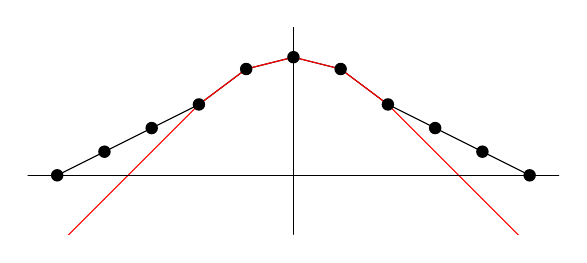
\begin{tikzpicture}[line cap=round,line join=round,>=triangle 45,scale=1.5]
      \clip(-2.25,-0.5) rectangle (2.25,1.25);
      \draw (0.4,0.9) -- (0.8,0.6);
      \draw (0.8,0.6) -- (1.2,0.4);
      \draw (1.2,0.4) -- (1.6,0.2);
      \draw (-0.4,0.9) -- (-0.8,0.6);
      \draw (-0.8,0.6) -- (-1.2,0.4);
      \draw (-1.2,0.4) -- (-1.6,0.2);
      \draw (-1.6,0.2) -- (-2,0);
      \draw (1.6,0.2) -- (2,0);
      \draw (-0.4,0.9) -- (0,1);
      \draw (0,1) -- (0.4,0.9);

      % New red curve aligning with black nodes
      \draw[red] (1.6,-.2) -- (2,-.6);
      \draw[red] (1.2,0.2) -- (1.6,-.2);
      \draw[red] (0.8,0.6) -- (1.2,0.2);
      \draw[red] (0.4,0.9) -- (0.8,0.6);
      \draw[red] (0,1) -- (0.4,0.9);
      \draw[red] (-0.4,0.9) -- (0,1);
      \draw[red] (-0.4,0.9) -- (-0.8,0.6);
      \draw[red] (-0.8,0.6) -- (-1.2,.2);
      \draw[red] (-1.2, .2) -- (-1.6,-.2);
      \draw[red] (-1.6,-.2) -- (-2,-.6);

      \begin{scriptsize}
        \fill [color=black] (-0.4,0.9) circle (1.5pt);
        \fill [color=black] (0.4,0.9) circle (1.5pt);
        \fill [color=black] (0.8,0.6) circle (1.5pt);
        \fill [color=black] (1.2,0.4) circle (1.5pt);
        \fill [color=black] (1.6,0.2) circle (1.5pt);
        \fill [color=black] (-0.8,0.6) circle (1.5pt);
        \fill [color=black] (-1.2,0.4) circle (1.5pt);
        \fill [color=black] (-1.6,0.2) circle (1.5pt);
        \fill [color=black] (-2,0) circle (1.5pt);
        \fill [color=black] (2,0) circle (1.5pt);
        \fill [color=black] (0,1) circle (1.5pt);
      \end{scriptsize}

      % Add Axes
      \draw[-] (-2.5,0) -- (2.5,0); % x-axis
      \draw[-] (0,-0.5) -- (0,1.45); % y-axis
    \end{tikzpicture}
    \caption{Iterate $u^k$(black) and obstacle $\psi$(red).}
  \end{subfigure}
  \hfill
  \begin{subfigure}[b]{.35\textwidth}
    \begin{tikzpicture}[line cap=round,line join=round,>=triangle 45,scale=1.5]
      \clip(-2.25,-0.5) rectangle (2.25,1.25);
      \draw (1.6,0) -- (2,0);
      \draw (1.2,0) -- (1.6,0);
      \draw (0.8,1) -- (1.2,0);
      \draw (0.4,1) -- (0.8,1);
      \draw (0,1) -- (0.4,1);
      \draw (-0.4,1) -- (0,1);
      \draw (-0.4,1) -- (-0.8,1);
      \draw (-0.8,1) -- (-1.2,0);
      \draw (-1.2,0) -- (-1.6,0);
      \draw (-1.6,0) -- (-2,0);

      % Add black vertices
      \begin{scriptsize}
        \fill [color=black] (1.6,0) circle (1.5pt);
        \fill [color=black] (2,0) circle (1.5pt);
        \fill [color=black] (1.2,0) circle (1.5pt);
        \fill [color=black] (0.8,1) circle (1.5pt);
        \fill [color=black] (1.2,0) circle (1.5pt);
        \fill [color=black] (0.4,1) circle (1.5pt);
        \fill [color=black] (0.8,1) circle (1.5pt);
        \fill [color=black] (0,1) circle (1.5pt);
        \fill [color=black] (0.4,1) circle (1.5pt);
        \fill [color=black] (-0.4,1) circle (1.5pt);
        \fill [color=black] (0,1) circle (1.5pt);
        \fill [color=black] (-0.4,1) circle (1.5pt);
        \fill [color=black] (-0.8,1) circle (1.5pt);
        \fill [color=black] (-1.2,0) circle (1.5pt);
        \fill [color=black] (-1.6,0) circle (1.5pt);
        \fill [color=black] (-2,0) circle (1.5pt);
      \end{scriptsize}
      
      % Add Axes
      \draw[-] (-2.5,0) -- (2.5,0); % x-axis
      \draw[-] (0,-0.5) -- (0,1.45); % y-axis
  
      % Label y=1
      \node at (-0.1,1.15) [left] {1};
      \draw[dashed] (-0.1,1) -- (0,1);
    \end{tikzpicture}
    \caption{Nodal active set indicator $s_0$.}
  \end{subfigure}
  \null\hfill
  \medskip

  \null\hfill
  \begin{subfigure}[b]{.35\textwidth}
    \centering
    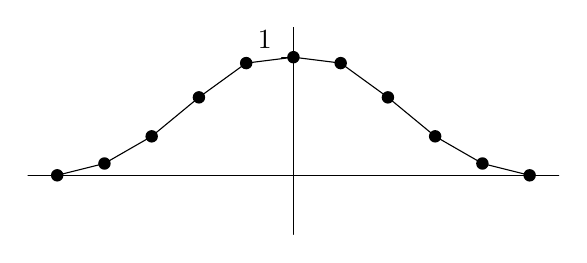
\begin{tikzpicture}[line cap=round,line join=round,>=triangle 45,scale=1.5]
      \clip(-2.25,-0.5) rectangle (2.25,1.25);
      
      % Draw the smoothed curve
      \draw (1.6, 0.1) -- (2,0);      
      \draw (1.2, 0.33) -- (1.6, 0.1);
      \draw (0.8, 0.66) -- (1.2, 0.33);
      \draw (0.4, 0.95) -- (0.8, 0.66);
      \draw (0,1) -- (0.4, 0.95);
      \draw (-0.4, 0.95) -- (0,1);
      \draw (-0.4, 0.95) -- (-0.8, 0.66);
      \draw (-0.8, 0.66) -- (-1.2, 0.33);
      \draw (-1.2, 0.33) -- (-1.6, 0.1);
      \draw (-1.6, 0.1) -- (-2,0);
  
      % Add black vertices
      \begin{scriptsize}
        \fill [color=black] (1.6, 0.1) circle (1.5pt);
        \fill [color=black] (2,0) circle (1.5pt);
        \fill [color=black] (1.2, 0.33) circle (1.5pt);
        \fill [color=black] (0.8, 0.66) circle (1.5pt);
        \fill [color=black] (0.4, 0.95) circle (1.5pt);
        \fill [color=black] (0,1) circle (1.5pt);
        \fill [color=black] (-0.4, 0.95) circle (1.5pt);
        \fill [color=black] (-0.8, 0.66) circle (1.5pt);
        \fill [color=black] (-1.2, 0.33) circle (1.5pt);
        \fill [color=black] (-1.6, 0.1) circle (1.5pt);
        \fill [color=black] (-2,0) circle (1.5pt);
      \end{scriptsize}
  
      % Add Axes
      \draw[-] (-2.5,0) -- (2.5,0); % x-axis
      \draw[-] (0,-0.5) -- (0,1.45); % y-axis
  
      % Label y=1
      \node at (-0.1,1.15) [left] {1};
      \draw[dashed] (-0.1,1) -- (0,1);
    \end{tikzpicture}
    \caption{Smoothed $s_1$.}
  \end{subfigure}
  \hfill
  \begin{subfigure}[b]{.35\textwidth}
    \centering
    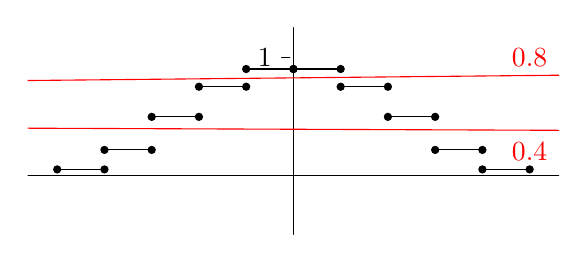
\begin{tikzpicture}[line cap=round,line join=round,>=triangle 45,scale=1.5]
      \clip(-2.25,-0.5) rectangle (2.25,1.25);

      % Draw horizontal segments at the heights of the calculated midpoints
      \draw (-2, 0.05) -- (-1.6, 0.05);
      \draw (-1.6, 0.215) -- (-1.2, 0.215);
      \draw (-1.2, 0.495) -- (-0.8, 0.495);
      \draw (-0.8, 0.75) -- (-0.4, 0.75);
      \draw (-0.4, 0.9) -- (0, 0.9);
      \draw (0, 0.9) -- (0.4, 0.9);
      \draw (0.4, 0.75) -- (0.8, 0.75);
      \draw (0.8, 0.495) -- (1.2, 0.495);
      \draw (1.2, 0.215) -- (1.6, 0.215);
      \draw (1.6, 0.05) -- (2, 0.05);

      % Add black vertices
      \begin{scriptsize}
        \fill [color=black] (-2, 0.05) circle (1pt);
        \fill [color=black] (-1.6, 0.05) circle (1pt);
        \fill [color=black] (-1.6, 0.215) circle (1pt);
        \fill [color=black] (-1.2, 0.215) circle (1pt);
        \fill [color=black] (-1.2, 0.495) circle (1pt);
        \fill [color=black] (-0.8, 0.495) circle (1pt);
        \fill [color=black] (-0.8, 0.75) circle (1pt);
        \fill [color=black] (-0.4, 0.75) circle (1pt);
        \fill [color=black] (-0.4, 0.9) circle (1pt);
        \fill [color=black] (0, 0.9) circle (1pt);
        \fill [color=black] (0, 0.9) circle (1pt);
        \fill [color=black] (0.4, 0.9) circle (1pt);
        \fill [color=black] (0.4, 0.75) circle (1pt);
        \fill [color=black] (0.8, 0.75) circle (1pt);
        \fill [color=black] (0.8, 0.495) circle (1pt);
        \fill [color=black] (1.2, 0.495) circle (1pt);
        \fill [color=black] (1.2, 0.215) circle (1pt);
        \fill [color=black] (1.6, 0.215) circle (1pt);
        \fill [color=black] (1.6, 0.05) circle (1pt);
        \fill [color=black] (2, 0.05) circle (1pt);
      \end{scriptsize}

      % Add Axes
      \draw[-] (-2.5,0) -- (2.5,0); % x-axis
      \draw[-] (0,-0.5) -- (0,1.25); % y-axis

      % Label y=1
      \node at (-0.1, 1) [left] {1};
      \draw[dashed] (-0.1, 1) -- (0, 1);

      % Add red horizontal lines at heights 0.8 and 0.4
      \draw[red] (-2.5, 0.8) -- (2.5, 0.85); % red line at y = 0.8
      \draw[red] (-2.5, 0.4) -- (2.5, 0.38);  % red line at y = 0.4
      % Label the heights of the red lines
      \node[red] at (2, 1) {0.8};
      \node[red] at (2, 0.2) {0.4};
    \end{tikzpicture}
    \caption{$interpolate(s_1,W)$. Threshold values in red.}
  \end{subfigure}
  \null\hfill
  \medskip

  \begin{subfigure}[b]{0.9\textwidth}
    \centering
    \begin{tikzpicture}[line cap=round,line join=round,>=triangle 45,scale=1.5]
      \clip(-2.5,-0.5) rectangle (2.5,1.25);
      
      \draw (1.6,0) -- (2,0);      
      \draw (1.2,0) -- (1.6,0);
      \draw (0.8,1) -- (1.2,1);
      \draw (0.4,1) -- (0.8,1);
      \draw (0,0) -- (0.4,0);
      \draw (-0.4,0) -- (0,0);
      \draw (-0.4,1) -- (-0.8,1);
      \draw (-0.8,1) -- (-1.2,1);
      \draw (-1.2,0) -- (-1.6,0);
      \draw (-1.6,0) -- (-2,0);
  
      % Add Axes
      \draw[-] (-2.5,0) -- (2.5,0); % x-axis
      \draw[-] (0,-0.5) -- (0,1.45); % y-axis
  
      % Label y=1
      \node at (-0.1, 1) [left] {1};
      \draw (-0.1, 1) -- (0, 1);
  
      % Add Nodes
      \begin{scriptsize}
      \fill [color=black] (1.6,0) circle (1.5pt);
      \fill [color=black] (2,0) circle (1.5pt);      
      \fill [color=black] (1.2,0) circle (1.5pt);
      \fill [color=black] (0.8,1) circle (1.5pt);
      \fill [color=black] (1.2,1) circle (1.5pt);
      \fill [color=black] (0.4,1) circle (1.5pt);
      \fill [color=black] (0.8,1) circle (1.5pt);
      \fill [color=black] (0,0) circle (1.5pt);
      \fill [color=black] (0.4,0) circle (1.5pt);
      \fill [color=black] (-0.4,0) circle (1.5pt);
      \fill [color=black] (0,0) circle (1.5pt);
      \fill [color=black] (-0.4,1) circle (1.5pt);
      \fill [color=black] (-0.8,1) circle (1.5pt);
      \fill [color=black] (-1.2,1) circle (1.5pt);
      \fill [color=black] (-1.2,0) circle (1.5pt);
      \fill [color=black] (-1.6,0) circle (1.5pt);
      \fill [color=black] (-2,0) circle (1.5pt);
      \end{scriptsize}
    \end{tikzpicture}
    \caption{Refinement indicator function $I$.}
  \end{subfigure}
  \vspace*{.25cm}
  \caption{Illustration of Variable Coefficient Elliptic Smoothing algorithm.}
\end{figure}

Support for unstructured meshes in Firedrake comes from the DMPlex class in PETSc, as developed by \citet{lange_flexible_2015}. DMPlex is a data management object which can store the topology (connectivity of mesh entities) and geometry (coordinates) of a discretization. In the DMPlex object every mesh entity is assigned a unique index. The connectivity of a mesh is stored as a layered directed acyclic graph (DAG) in which a "covering" relation specifies the edges of the graph. For example, for a tetrahedral element in a 3d mesh, a face is covered by 3 edges and a tetrahedral cell is covered by 4 faces. Each layer represents a class of mesh entity i.e vertices, edges, etc. Below is an example of how a single tetrahedral cell is represented by DMPlex.

The DMPlex object has several methods which make querying the mesh topology and geometry simple \citep{lange_efficient_2016}. For example, let $p$ be an index assigned by DMPlex. Then $\emph{cone}(p)$ returns all the in-neighbors of $p$. In the example above $\emph{cone}(0) = \{11, 12, 13, 14\}$. The transitive closure of $\emph{cone}(p)$ is also available with $\emph{closure}(p)$. The dual of $\emph{cone}(p)$ is $\emph{support}(p)$ which returns all the out-neighbors of $p$. In the example above $\emph{support}(6) = \{6, 7, 10\}$. The transitive closure of $\emph{support}(p)$ is also available with $\emph{star}(p)$. 

The use of DMPlex queries is essential to our second strategy, the Unstructured Dilation Operator (UDO). We identify the set $B$ of elements that border the computed free boundary $\Gamma_{u^k}$ by interpolating a nodal active indicator function into DG0 and thresholding for values in the range (0, 1). We then use the \emph{closure} and \emph{star} methods to create vertex-to-cell and cell-to-vertex mappings. These mappings are then used to determine which elements are neighbors to the computed free boundary. We say an element neighbors another if it shares at least one vertex. The function $N(\triangle)$ returns a set of elements:
\begin{equation}
  N(\triangle) = \{\triangle_i \in T: \triangle \text{ shares at least 1 vertex with } \triangle_i\}.
\end{equation}
This process is then repeated $n$ times to create a set of elements that are within $n$ neighborhood levels of the border elements:
\begin{equation}
  N^n(\triangle) = \underbrace{N(...N(\triangle))}_{n \text{ times}}.
\end{equation}
As show in Algorithim 3, for a border element set $B$, defined below in (5.5) we use breadth-first search to construct the set $N^n(B)$ and then assemble its corresponding indicator function. This process expand the support of the DG0 indicator function in a way that resembles the "dilation" operation in image processing as seen in \citep{OpenCV} but it is applied over an unstructured mesh.

\begin{algorithm}[H]
  \caption{Unstructured Dilation Operator Element Tagging for VIs}
  \begin{algorithmic}[1]
    \Require $tol \in \mathbb{R}$, $u^k \in K, \psi \in V$, $W$ is a DGO FE space, mesh $T$.
    \Require Neighborhood Depth Parameter $n \in \mathbb{N}$.
    \State Compute the nodal active set indicator function $s$
    \begin{equation}
    s = \begin{cases}
      1 & \text{ if } u^k - \psi < tol\\
      0 & \text{ otherwise}
    \end{cases}.
    \end{equation}
  
    \State Let $s_W = interpolate(s, W)$ .
    \State Define the border element set $B$:
    \begin{equation}
    B = \{\triangle \in T: 0 < s_W(\triangle) < 1 \} .
    \end{equation}

    \State Use the \emph{closure} and \emph{star} methods to construct vertex-to-cell and cell-to-vertex mappings.

    \State Use breadth-first search to construct the set $N^n(B)$ as in (5.2) and (5.3). 
    \State Assemble the indicator function $I$ of the set $N^n(B)$. \\
    \Return $I$
  \end{algorithmic}
  \end{algorithm}

A simple example using UDO is shown.

%\inputminted{python}{short.py}

Using thresholding $u - \psi < 0.001$ to determine the active set, running this example generates the following Figure.

\begin{figure}[H]
FIXME
\caption{Mesh (left) generated from the spiral problem, with $N=2.3\times 10^3$ elements, and the approximated active set (right).}
\end{figure}


\section{Results} \label{sec:results}

FIXME discuss norm and geometric measures first

FIXME \cite{Kosub2016} \cite{JungeblutKleistMiltzow2022}

FIXME

\section{Application to determining glaciated areas} \label{sec:app}


FIXME

%\section*{Acknowledgements}

%\section*{Notes on contributor(s)}
%An unnumbered section, e.g.\ \verb"\section*{Notes on contributors}", may be included \emph{in the non-anonymous version} if required. A photograph may be added if requested.


\section{References}

\bibliographystyle{tfs}
\bibliography{viamr}


%Any appendices should be placed after the list of references, beginning with the command \verb"\appendix" followed by the command \verb"\section" for each appendix title, e.g.
%\appendix
%\section{This is the title of the first appendix}

\end{document}
